\documentclass[12pt,fleqn]{article}
\usepackage{fullpage}
\usepackage{amsmath}
\usepackage{multirow}
\usepackage{graphicx}
\usepackage{indentfirst}
\usepackage{multicol}
\title{\LARGE \textbf{Trabajo práctico 3}}
\author{Martín Rossi}
\date{}
\begin{document}
\maketitle
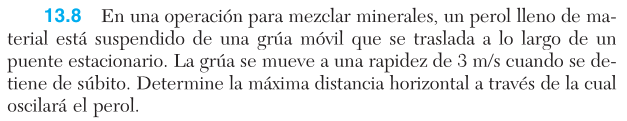
\includegraphics[width=\linewidth]{13.8}
\begin{center}
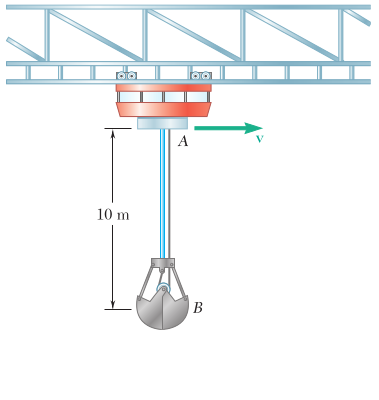
\includegraphics[width=200px]{13.8.0}
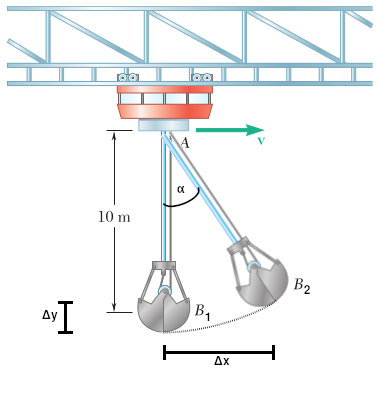
\includegraphics[width=200px]{13.8.1}
\end{center}

$B_1$ es cuando se frena la grúa y el perol tiene una rapidez de $v=3$ $m/seg$. $B_2$ cuando llega al punto máximo en la oscilación y $v=0$.\\

La energía cinética en $B1$ es $T_1=\frac{1}{2}*m*3^2=\frac{9}{2}*m$ J. Y en $B2$, $T_2=0$.

Por lo tanto por el principio de trabajo y energía $U_{1\rightarrow 2}=T_2-T_1=-\frac{9}{2}*m$ J. (1)

\begin{center}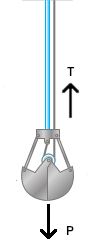
\includegraphics[width=50px]{13.8.2}\end{center}

Las fuerzas que actúan sobre el perol son el peso $P$ y la tensión del cable $T$.

$T$ no realiza trabajo porque es perpendicular a la trayectoria. La única fuerza que lo realiza es $P$ que es siempre vertical y se calcula como $U_{1\rightarrow 2}=P*\Delta y=m*g*\Delta y$ J. (2)\\

Igualando (1) y (2) queda $m*g*\Delta y=-\frac{9}{2}*m \implies \Delta y=-0.4592$ m.\\

Sabiendo el desplazamiento en el eje vertical se calcula en el horizontal:

cos$(\alpha)=\frac{10-0.4592}{10}=0.95408$

sin$(\alpha)=0.2996=\frac{\Delta x}{10}\implies \mathbf{\Delta x=2.996}$ \textbf{m}
\newpage
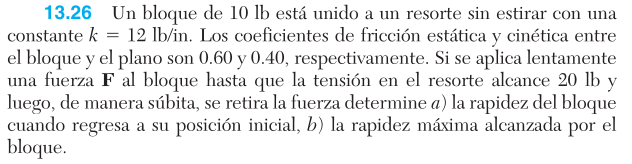
\includegraphics[width=\linewidth]{13.26}
\begin{center}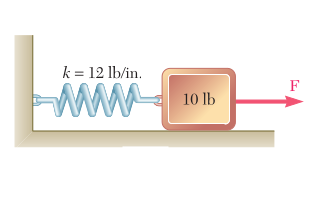
\includegraphics[width=200px]{13.26.1}\end{center}
\subsubsection*{a)}
\begin{center}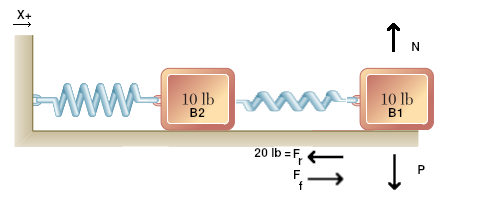
\includegraphics[width=300px]{13.26.0}\end{center}

La tensión del resorte $F_r$ se calcula como $F_r=k*x$, con $k$ la constante del resorte y $x$ la deformación. Entonces $20=F_r=12*x \implies x=\frac{5}{3}$ in\\

\textbf{Fuerza del resorte}:

El resorte tiene una tensión de 20 lb cuando se suelta y llega hasta la posición inicial donde la tensión es 0.

Usando la fórmula para el trabajo $U_{1\rightarrow 2}=\frac{1}{2}*k*x_1^2-\frac{1}{2}*k*x_2^2$ se obtiene:

$(U_{1\rightarrow 2})_r=\frac{1}{2}*12*\frac{5}{3}^2-\frac{1}{2}*12*0=\frac{50}{3}$ lb*in\\

\textbf{Fuerza de fricción}:

$F=N*\mu_k=10*0.4=4$ lb

$(U_{1\rightarrow 2})_f=F*x=4*(-\frac{5}{3})=-\frac{20}{3}$ lb*in\\

El trabajo total es $U_{1\rightarrow 2}=(U_{1\rightarrow 2})_f+(U_{1\rightarrow 2})_r=\frac{50}{3}-\frac{20}{3}=10$ lb*in (1)\\

Por el principio de trabajo y energía $U_{1\rightarrow 2}=T_2-T_1=\frac{1}{2}*m*v_2^2$ (2), donde $v_2$ será la rapidez con la que pasa por la posición inicial.\\

Igualando (1) y (2):

$\frac{1}{2}*m*v_2^2=10\implies \frac{10}{386.088}*v_2^2=20\implies \mathbf{v_2=27.79}$ \textbf{in/seg}$\mathbf{=2.32}$ \textbf{ft/seg}
\subsubsection*{b)}
El punto de rapidez máxima será cuando la aceleración sea 0. Se calcula la posición de este bloque $B_3$ con la segunda ley de Newton:
\begin{align*}
  F&=m*a\\
  F&=0\tag{a=0}\\
  F_r+F_f&=0\tag{Fuerzas de fricción y del resorte}\\
  -k*x+N*\mu_k&=0\\
  -12*x+10*0.4&=0\\
  x&=\frac{1}{3}\textrm{ in}
\end{align*}

\textbf{Fuerza del resorte}:

$(U_{1\rightarrow 3})_r=\frac{1}{2}*12*\frac{5}{3}^2-\frac{1}{2}*12*\frac{1}{3}^2=16$ lb*in\\

\textbf{Fuerza de fricción}:

$F=N*\mu_k=10*0.4=4$ lb

$(U_{1\rightarrow 3})_f=F*x=4*(\frac{1}{3}-\frac{5}{3})=-\frac{16}{3}$ lb*in\\

El trabajo total es $U_{1\rightarrow 3}=(U_{1\rightarrow 3})_f+(U_{1\rightarrow 3})_r=\frac{32}{3}$ lb*in (1)\\

Por el principio de trabajo y energía $U_{1\rightarrow 3}=T_3-T_1=\frac{1}{2}*m*v_3^2$ (2)\\

Igualando (1) y (2):

$\frac{1}{2}*m*v_3^2=\frac{32}{3}\implies \mathbf{v_3=28.69}$ \textbf{in/seg}$=\mathbf{2.39}$ \textbf{ft/seg}
\newpage
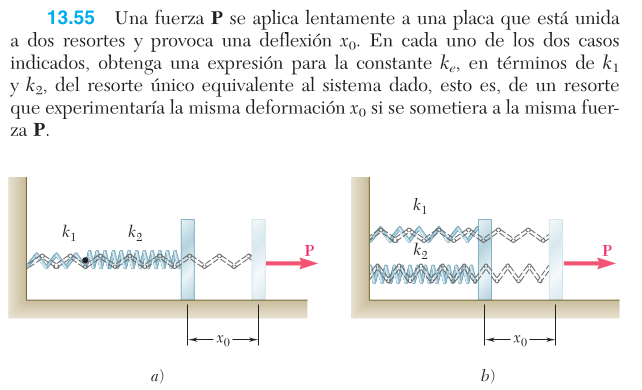
\includegraphics[width=\linewidth]{13.55}
\subsubsection*{a)}
Los dos resortes están enganchados. Si sus deformaciones son $x_1$ y $x_2$ para el resorte con $k_1$ y $k_2$, entonces $x_1+x_2=x_0$. (1)\\

La fuerza del resorte equivalente $F_e$ es igual a $P$.

$F_e=-k_e*x_0=P\implies x_0=-\frac{P}{k_e}$\\

$P$ es también igual a $F_1$ y a $F_2$, las tensiones de cada uno de los resortes.

$F_1=-k_1*x_1=P\implies x_1=-\frac{P}{k_1}$

$F_2=-k_2*x_2=P\implies x_2=-\frac{P}{k_2}$\\

Por lo tanto reemplazando los valores de $x_0$, $x_1$ y $x_2$ en (1):
\begin{align*}
  \frac{P}{k_e}&=\frac{P}{k_1}+\frac{P}{k_2}\\
  \frac{1}{k_e}&=\frac{1}{k_1}+\frac{1}{k_2}\\
  \frac{1}{k_e}&=\frac{k_2+k_1}{k_1*k_2}\\
  \mathbf{k_e}&=\mathbf{\frac{k_1*k_2}{k_1+k_2}}
\end{align*}
\subsubsection*{b)}
Cada resorte se alarga $x_0$. La fuerza $F_e$ del resorte equivalente es $P$, y ahora la suma de los resortes en paralelo es $F_1+F_2=P$.
\begin{align*}
  P&=F_1+F_2\\
  -k_e*x_0&=-k_1*x_0-k_2*x_0\\
  -k_e*x_0&=-(k_1+k_2)*x_0\\
  \mathbf{k_e}&\mathbf{=k_1+k_2}
\end{align*}
\end{document}